\documentclass[12pt,a4paper]{article}

\usepackage[margin=2.5cm]{geometry}
\usepackage{setspace}
\usepackage{parskip}
\usepackage{titlesec}
\usepackage{tocloft}
\usepackage{hyperref}
\usepackage{microtype}
\usepackage{booktabs}
\usepackage{array}
\usepackage{enumitem}
\usepackage{fancyhdr}
\usepackage{amsmath}
\usepackage{graphicx}
\usepackage{xcolor}
\usepackage{listings}
\usepackage{caption}
\usepackage{float}
\usepackage{tikz}
\usetikzlibrary{arrows.meta,positioning}

\hypersetup{
  colorlinks=true,
  linkcolor=black,
  urlcolor=blue,
  citecolor=black
}

\definecolor{codebg}{HTML}{F7F8FA}
\definecolor{codeborder}{HTML}{D7DDE6}
\definecolor{codekw}{HTML}{1F4E79}
\definecolor{codestring}{HTML}{8A3A21}
\definecolor{codecomment}{HTML}{68707D}
\definecolor{codenumber}{HTML}{8A93A3}
\definecolor{diagramline}{HTML}{607087}
\definecolor{diagramfill}{HTML}{F6F8FB}
\definecolor{diagramaccent}{HTML}{1F4E79}

\lstdefinelanguage{Solidity}{
  keywords={
    address,bool,uint256,string,memory,calldata,storage,external,public,private,
    internal,view,pure,payable,immutable,contract,enum,struct,event,modifier,
    require,emit,return,returns,function,if,for,while,else,true,false
  },
  sensitive=true,
  morecomment=[l]{//},
  morecomment=[s]{/*}{*/},
  morestring=[b]",
}

\lstdefinelanguage{TypeScript}{
  keywords={
    const,let,var,function,return,if,else,await,async,import,export,from,type,
    interface,extends,as,true,false,null,undefined,new,class,try,catch,throw
  },
  sensitive=true,
  morecomment=[l]{//},
  morecomment=[s]{/*}{*/},
  morestring=[b]",
  morestring=[b]',
  morestring=[b]`,
}

\lstdefinestyle{solidity}{
  language=Solidity,
  backgroundcolor=\color{codebg},
  basicstyle=\ttfamily\scriptsize,
  keywordstyle=\color{codekw}\bfseries,
  commentstyle=\color{codecomment}\itshape,
  stringstyle=\color{codestring},
  breaklines=true,
  breakatwhitespace=true,
  columns=fullflexible,
  keepspaces=true,
  frame=single,
  framerule=0.35pt,
  rulecolor=\color{codeborder},
  framesep=4pt,
  xleftmargin=6pt,
  xrightmargin=6pt,
  numbers=none,
  showstringspaces=false,
  tabsize=2,
  aboveskip=5pt,
  belowskip=5pt,
  captionpos=b
}

\lstdefinestyle{typescript}{
  language=TypeScript,
  backgroundcolor=\color{codebg},
  basicstyle=\ttfamily\scriptsize,
  keywordstyle=\color{codekw}\bfseries,
  commentstyle=\color{codecomment}\itshape,
  stringstyle=\color{codestring},
  breaklines=true,
  breakatwhitespace=true,
  columns=fullflexible,
  keepspaces=true,
  frame=single,
  framerule=0.35pt,
  rulecolor=\color{codeborder},
  framesep=4pt,
  xleftmargin=6pt,
  xrightmargin=6pt,
  numbers=none,
  showstringspaces=false,
  tabsize=2,
  aboveskip=5pt,
  belowskip=5pt,
  captionpos=b
}

\pagestyle{fancy}
\fancyhf{}
\rhead{DealLock --- FTE4312 Final Report}
\lhead{}
\cfoot{\thepage}
\renewcommand{\headrulewidth}{0.4pt}
\setlength{\headheight}{15pt}

\titleformat{\section}{\large\bfseries}{\thesection}{1em}{}
\titleformat{\subsection}{\normalsize\bfseries}{\thesubsection}{1em}{}
\titleformat{\subsubsection}{\normalsize\itshape}{\thesubsubsection}{1em}{}

\titlespacing*{\section}{0pt}{14pt}{5pt}
\titlespacing*{\subsection}{0pt}{10pt}{4pt}

\setlist[itemize]{topsep=3pt, itemsep=1pt}
\setlist[enumerate]{topsep=3pt, itemsep=1pt}

\setstretch{1.45}
\emergencystretch=3em

% Compact table of contents with enough spacing for readable entries.
\setlength{\cftbeforesecskip}{0.68em}
\setlength{\cftbeforesubsecskip}{0.22em}

\begin{document}

% -----------------------------------------------------------------------
% Title page
% -----------------------------------------------------------------------
\begin{titlepage}
  \centering
  \vspace*{1.2cm}
  {\LARGE \textbf{DealLock}\\[6pt]}
  {\large A Milestone-Based Escrow dApp for Digital Freelance Deliverables\\[0.8cm]}
  {\normalsize FTE4312 --- Course Project Final Report\\[0.4cm]}
  {\normalsize April 2026\\[1.2cm]}
  {\normalsize
    Ho Dang Dung (Student ID: 325040027)\\[0.25cm]
    Taisiia Ibragimova (Student ID: 325040033)\\[0.45cm]
  }
  \vfill
  \begin{abstract}
    \noindent
    DealLock is a browser-native dApp for milestone-based escrow in structured
    digital freelance agreements. One Solidity contract represents one agreement
    between a client and a provider, holding native ETH and enforcing acceptance,
    exact funding, sequential submission, approval, and refund of expired pending
    milestones. The React/Vite frontend uses wagmi and viem to deploy and operate
    contracts on Sepolia, while optional titles, notes, and agreement history stay
    in browser \texttt{localStorage}. Evaluation is based on an eleven-case
    Hardhat test suite covering the reachable contract state transitions and a
    Sepolia-oriented demo workflow. The project is intentionally scoped as an MVP:
    it enforces payment flow, not subjective quality judgement or arbitration.
  \end{abstract}
\end{titlepage}

\begingroup
\singlespacing
\setlength{\parskip}{0pt}
\tableofcontents
\endgroup
\clearpage

% -----------------------------------------------------------------------
% 1. Introduction
% -----------------------------------------------------------------------
\section{Introduction}

Freelance digital work is often paid in a lump sum at project completion, which
creates an asymmetric risk that benefits neither party.
The client risks paying before delivery; the provider risks delivering without
payment. Milestone payments reduce this exposure by splitting a project into
phases, but informal milestone schedules in chats or shared documents remain
hard to enforce.

Smart contracts offer a different enforcement mechanism.
A self-executing program on a public blockchain can hold funds in escrow, release
them only when a defined condition is met, and refund them if a deadline passes
without action.
Unlike a paper agreement, the enforcement logic is automatic and does not require
either party to trust the other with custody of the funds.

DealLock applies this mechanism directly to digital freelance agreements.
Each agreement between a client and a provider is a separately deployed Solidity
contract instance.
The contract stores the milestone list, the escrowed funds, and the recorded
delivery references.
The React frontend lets either party connect MetaMask, deploy or load a contract,
and drive the workflow without a backend server.

The project was conceived as an MVP demonstration suitable for the Sepolia
public Ethereum testnet.
It targets a focused range of deliverable types: website and landing page
development, UI/UX design, and branding or logo packages --- service relationships
where handoffs are discrete, evidence is linkable, and the workflow phases are
easy to specify in advance.
This narrower framing is important because the contract enforces workflow and
fund movement, not subjective judgements about design quality or scope changes.

\newpage
% -----------------------------------------------------------------------
% 2. Background
% -----------------------------------------------------------------------
\section{Background}
\label{sec:background}

\subsection{Escrow in digital service delivery}

An escrow arrangement places funds under the custody of a neutral party or
mechanism until a condition is satisfied.
In traditional digital freelance platforms such as Upwork or Fiverr, the platform
itself acts as the escrow agent: money is deposited before work starts and released
when the client marks the order complete.
This model works but depends on the platform's rules, custody, fees, and dispute
process.

A milestone structure distributes risk further: the provider knows funds are
locked before work begins, while the client releases only the tranche attached
to a submitted and accepted deliverable.

\subsection{Smart contracts as enforcement}

Ethereum's programmable account model allows deploying bytecode to a
deterministic address on the blockchain.
A smart contract executes exactly as written; there is no way for either party
--- or any third party, including the original deployer --- to alter the execution
path once the code is deployed.
State changes (fund transfers, milestone approvals) are recorded permanently in
the chain, are visible to both parties via a block explorer, and require the
designated signer's private key.
This makes smart contracts a useful primitive for escrow logic, with one
important trade-off: the code can enforce state transitions and payments, but it
cannot judge whether the delivered work is satisfactory.

\subsection{MVP rationale and scope}

The project therefore focuses on the smallest complete escrow loop: staged
payments, delivery reference recording, client approval, and refund after
deadline expiry. Avoiding a backend keeps the trust model simple: binding terms
are on-chain, while non-binding titles and notes remain in the browser.

\newpage
% -----------------------------------------------------------------------
% 3. System Architecture
% -----------------------------------------------------------------------
\section{System Architecture}
\label{sec:architecture}

\subsection{Overview}

DealLock is a client-only decentralised application (dApp).
Figure~\ref{fig:arch} outlines the two main layers: the user's browser running
the React application, and the Ethereum network hosting deployed contract instances.

\begin{figure}[H]
\centering
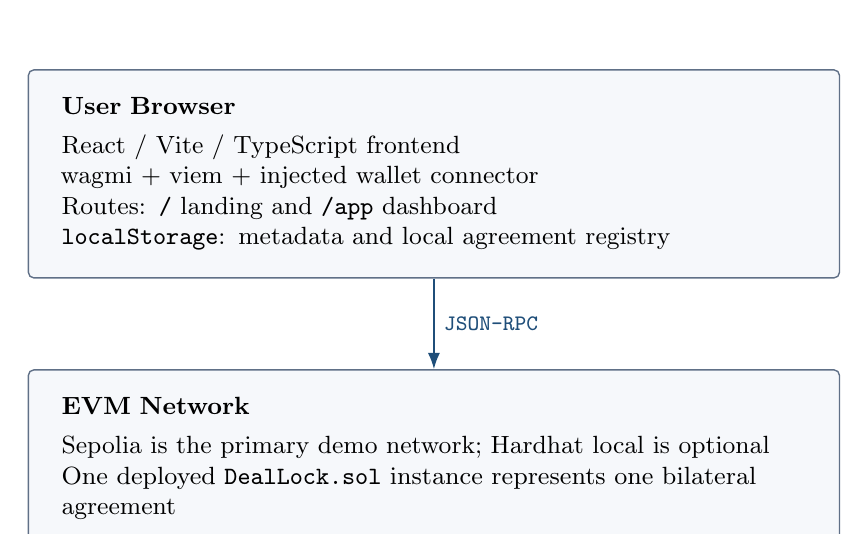
\begin{tikzpicture}[
  font=\small,
  box/.style={
    draw=diagramline,
    rounded corners=2pt,
    fill=diagramfill,
    line width=0.5pt,
    align=left,
    inner xsep=12pt,
    inner ysep=10pt,
    text width=0.78\textwidth
  },
  arrow/.style={-Latex, line width=0.65pt, draw=diagramaccent}
]
  \node[box] (browser) {
    \textbf{User Browser}\\[3pt]
    React / Vite / TypeScript frontend\\
    wagmi + viem + injected wallet connector\\
    Routes: \texttt{/} landing and \texttt{/app} dashboard\\
    \texttt{localStorage}: metadata and local agreement registry
  };

  \node[box, below=1.15cm of browser] (chain) {
    \textbf{EVM Network}\\[3pt]
    Sepolia is the primary demo network; Hardhat local is optional\\
    One deployed \texttt{DealLock.sol} instance represents one bilateral agreement
  };

  \draw[arrow] (browser.south) -- node[right, font=\footnotesize\ttfamily, text=diagramaccent] {JSON-RPC} (chain.north);
\end{tikzpicture}
\caption{High-level system architecture.}
\label{fig:arch}
\end{figure}

There is no backend, no application server, no database, and no factory contract.
Each deployment of \texttt{DealLock.sol} represents exactly one agreement between
one client and one provider.
The only off-chain persistence is the browser's \texttt{localStorage} API, which
holds optional agreement metadata (project title, service template, guidance notes)
and a browser-local registry of contracts the user has created or loaded.

\subsection{Main layers}

The smart contract is Solidity~\verb|^0.8.20| compiled by Hardhat~3 with the
optimizer enabled. Construction fixes the client as the deployer, stores the
provider address, and writes parallel arrays of milestone descriptions, amounts,
and deadlines. These terms are not editable after deployment.

The frontend is a React~19, TypeScript, Vite~6 single-page app using wagmi~2,
viem, and TanStack Query. Wallet connection uses the injected provider
(MetaMask in the demo). Sepolia is listed first in \texttt{wagmi.ts}; Hardhat
local remains available for development through the Vite \texttt{/rpc-hardhat}
proxy. Mainnet is intentionally omitted.

\subsection{Separation of on-chain and off-chain data}

The design draws a clear line between what is stored on-chain and what is stored
in the browser:

\begin{table}[H]
\centering
\small
\renewcommand{\arraystretch}{1.3}
\begin{tabular}{p{0.44\textwidth} p{0.44\textwidth}}
\toprule
\textbf{On-chain (DealLock.sol)} & \textbf{Browser only (localStorage)} \\
\midrule
Client and provider addresses & Project title \\
Total amount, funded/released/refunded amounts & Service template choice \\
Agreement state & Evidence / acceptance guidance notes \\
Milestone descriptions, amounts, deadlines & Per-milestone notes \\
Milestone state, proof string, submission timestamp & Agreement registry (addresses seen, sort order) \\
 & Sidebar role filter setting \\
\bottomrule
\end{tabular}
\caption{Data separation between on-chain contract state and browser-local storage.}
\label{tab:data}
\end{table}

The contract is the canonical source of truth for all binding agreement terms.
The \texttt{localStorage} data is advisory and UI-enhancement only; it is not
shared across browsers or devices, and losing it does not affect the ability to
operate the agreement through a different browser.

\newpage
% -----------------------------------------------------------------------
% 4. Workflow and Design Description
% -----------------------------------------------------------------------
\section{Workflow and Design Description}
\label{sec:workflow}

\subsection{Application flow}

The frontend has two routes: \texttt{/} for the landing page and \texttt{/app}
for the working dashboard. The dashboard has a browser-local ``My agreements''
sidebar and a main workspace. With no contract selected, the workspace offers
Create and Load modes; with a contract selected, it shows the role, state,
parties, ETH totals, available actions, milestone timeline, and saved context.

Creating an agreement is gated by wallet connection and supported-chain checks.
The form collects:
\begin{itemize}
  \item a service template and project title, stored only as local metadata;
  \item The provider's Ethereum address.
  \item per-milestone description, ETH amount, future deadline, and optional note.
\end{itemize}

The client-side checks mirror constructor constraints: valid provider address,
at least one milestone, positive amounts, future deadlines, and non-decreasing
deadline order. Deployment uses the browser wallet to submit contract creation
bytecode; the UI then records the new address and metadata in \texttt{localStorage}.
Loading an existing agreement only requires a contract address. The dashboard
validates the address, stores it in the local registry, and reads party, state,
balance, and milestone data from the chain. Wrong-network and wrong-address
cases are surfaced as dashboard banners.

\subsection{Contract lifecycle}

The on-chain lifecycle is:
\begin{enumerate}
  \item \textbf{Proposed}: contract is deployed; provider has not accepted.
  \item \textbf{Accepted}: provider accepted; client can fund exact total.
  \item \textbf{Funded}: escrow is active; provider submits, client approves or refunds.
  \item \textbf{Completed}: all milestone amounts are released or refunded.
\end{enumerate}
The enum also contains \texttt{Cancelled} for future extension, but the MVP does
not implement cancellation logic. Milestones are sequential: submitting or
approving milestone $i$ requires all earlier milestones to be Released, while
refund of milestone $i$ requires all earlier milestones to be resolved
(Released or Refunded). The action panel reflects those rules by showing only
the buttons the connected role can validly sign.

\subsection{Key design choices}

The key design choices follow from the MVP goal. One contract per agreement
keeps deployment and loading simple. Sepolia gives real wallet signing and public
Etherscan inspection without real funds. A backend is avoided so the trust model
stays clear: the contract is authoritative, and \texttt{localStorage} is only a
convenience layer for titles, templates, notes, filters, and agreement history.

\newpage
% -----------------------------------------------------------------------
% 5. Implementation Details
% -----------------------------------------------------------------------
\section{Implementation Details}
\label{sec:implementation}

\subsection{Smart contract (\texttt{DealLock.sol})}

The contract defines two state machines: agreement state
(\texttt{Proposed}, \texttt{Accepted}, \texttt{Funded}, \texttt{Completed},
\texttt{Cancelled}) and milestone state (\texttt{Pending}, \texttt{Submitted},
\texttt{Released}, \texttt{Refunded}). Each milestone stores description,
amount, deadline, proof string, submission time, and state. Agreement-level
storage tracks funded, released, and refunded totals, while \texttt{client},
\texttt{provider}, and \texttt{totalAmount} are immutable.

\begin{lstlisting}[style=solidity, caption={Core state model and entry points.}, label={lst:contract-core}]
enum AgreementState {
    Proposed,
    Accepted,
    Funded,
    Completed,
    Cancelled
}

enum MilestoneState {
    Pending,
    Submitted,
    Released,
    Refunded
}

function fundAgreement()
    external
    payable
    onlyClient
    inState(AgreementState.Accepted)
{
    require(msg.value == totalAmount, "Incorrect funding amount");
    fundedAmount = msg.value;
    agreementState = AgreementState.Funded;
    emit AgreementFunded(client, msg.value);
}

function approveMilestone(uint256 milestoneId)
    external
    onlyClient
    inState(AgreementState.Funded);
\end{lstlisting}

The constructor rejects a zero provider address, empty or mismatched milestone
arrays, empty descriptions, zero amounts, past deadlines, and unsorted deadlines.
Runtime access control is handled by \texttt{onlyClient}, \texttt{onlyProvider},
and \texttt{inState}. The contract also rejects direct ETH transfers through
\texttt{receive} and \texttt{fallback}, so funds enter only through
\texttt{fundAgreement}. Approval and refund update state before transferring ETH
with low-level \texttt{call}; completion is detected when released plus refunded
amounts equal \texttt{totalAmount}. Events record acceptance, funding,
submission, release, and refund.

\subsection{Hardhat configuration and tooling}

\texttt{hardhat.config.ts} uses the Hardhat~3 Mocha/Ethers toolbox, Solidity
0.8.20, optimizer runs set to 200, and tests under \texttt{test/}. Sepolia is
configured only when \texttt{SEPOLIA\_RPC\_URL} and \texttt{PRIVATE\_KEY} are
present, so local tests do not require network credentials.

\subsection{Frontend modules}

\texttt{main.tsx} installs the wagmi and React Query providers and routes
\texttt{/} to \texttt{LandingPage} and \texttt{/app} to \texttt{DashboardPage}.
\texttt{wagmi.ts} defines Sepolia-first transports, while \texttt{network.ts}
centralises chain IDs, explorer links, and \texttt{switchToSepolia}. The ABI and
browser deployment bytecode are exported from \texttt{contract.ts} and
\texttt{bytecode.ts}; the latter must be regenerated after contract changes.

The dashboard reads scalar contract fields with \texttt{useReadContract} and
milestones with \texttt{useReadContracts}, gated by wallet connection, supported
chain, and a valid contract address. \texttt{storage.ts} implements two
browser-only persistence layers: per-address metadata and a local agreement
registry. \texttt{types.ts} provides role derivation by comparing the connected
wallet with on-chain client/provider addresses. \texttt{templates.ts} supplies
off-chain service templates; they prefill UI guidance but do not change
constructor arguments.

The main interaction components cover creation, actions, milestones, overview,
and the agreement sidebar. They expose only actions valid for the connected role
and contract state: provider accept/submit, client fund/approve/refund, or
read-only display for unrelated wallets. Transaction states are shown as pending,
confirming, success, or error, with Sepolia Etherscan links where available.

\subsection{Test suite (\texttt{test/DealLock.ts})}

The test suite uses Mocha and the Hardhat~3 network helpers with the ethers
plugin.
Tests run against a local in-memory Hardhat chain only; no network credentials
are required.
The fixture \texttt{deployDealLockFixture} deploys a three-milestone agreement
(Prototype, Beta, Final at 1/2/3 ETH with deadlines 100/200/300 seconds into the
future) using three signers: \texttt{client}, \texttt{provider}, and
\texttt{other}.

The eleven tests cover deployment state, provider-only acceptance, exact funding,
submission after funding, sequential submission, approval payout, rejection of
unsubmitted approval, expired refunds, early-refund rejection, sequential refund
ordering, and full completion. They assert revert reasons, emitted events, and
Ether balance changes for release/refund paths.

\newpage
% -----------------------------------------------------------------------
% 6. Evaluation / Results
% -----------------------------------------------------------------------
\section{Evaluation and Results}
\label{sec:evaluation}

\subsection{Smart contract correctness}

The Hardhat test suite was run against the final version of the contract.
All eleven tests pass.
The suite exercises the reachable state transitions and access-control
boundaries: only the provider can accept, only the client can fund/approve/refund,
funding must match \texttt{totalAmount}, milestones cannot be submitted out of
order, approval transfers the correct amount to the provider, refunds are allowed
only after deadline expiry, and completion is reached after all milestones are
released. No unexpected reverts or state inconsistencies were observed.

\subsection{End-to-end application workflow}

The repository also contains a Sepolia runbook for a two-wallet demo: client
deploys, provider accepts, client funds, provider submits evidence, and client
approves or refunds until completion. The frontend follows this lifecycle and
adds Etherscan links for Sepolia transaction hashes and addresses. The report
does not present performance numbers because no benchmark data was collected.

\subsection{Error path coverage}

The frontend handles common demo failures: unsupported chains trigger a switch
prompt; wallet addresses or wrong-chain contract addresses produce a readable
``no DealLock data'' message; missing Hardhat local RPC returns an explanatory
JSON-RPC error; and wallets that are neither client nor provider see a read-only
state instead of write buttons.

\subsection{Demo readiness and practical usability}

The application is suitable for a live classroom demo. The sidebar supports quick
switching between agreements, the header shows role/state/ETH progress, and
pending/confirming/success/error states make public-testnet delays understandable.

\newpage
% -----------------------------------------------------------------------
% 7. Limitations and Future Work
% -----------------------------------------------------------------------
\section{Limitations and Future Work}
\label{sec:limitations}

\subsection{Limitations of the current MVP}

DealLock's limitations come directly from the MVP scope. The local agreement
registry and metadata are browser-only, so users must keep the contract address
if they switch devices or clear browser storage. The contract has no arbitration
or proof-quality oracle: it checks that a proof string exists, but not whether a
link works or the delivered work is good. It supports native ETH only, not ERC-20
tokens or stablecoins. There is also no factory, marketplace, indexer, global
agreement search, or on-chain revision workflow; milestone terms are fixed at
deployment. Finally, one deployment per agreement is easy to understand but would
be inefficient for a production marketplace with many agreements.

\subsection{Future work}

Useful extensions would be an event indexer or factory contract for agreement
discovery, optional mediator-based dispute resolution, ERC-20 or stablecoin
payments, cross-device metadata sync through wallet-signed writes, and a more
structured proof format such as URL plus content hash. These additions would move
DealLock from a classroom escrow MVP toward a more practical product while
preserving the same core state machine.

\newpage
% -----------------------------------------------------------------------
% 8. Member Contribution Statement
% -----------------------------------------------------------------------
\section{Member Contribution Statement}
\label{sec:contributions}

The project was completed by a group of two students, as registered on the
FTE4312 project proposal.
The following table summarises each member's primary areas of responsibility.

\begin{table}[H]
\centering
\renewcommand{\arraystretch}{1.4}
\small
\begin{tabular}{p{0.22\textwidth} p{0.68\textwidth}}
\toprule
\textbf{Member} & \textbf{Contributions} \\
\midrule
Ho Dang Dung\newline\footnotesize{(325040027)}
& Smart contract design and implementation (\texttt{DealLock.sol}); Hardhat
  configuration; Mocha test suite; CLI deploy script; contract ABI and bytecode
  wiring for the frontend. \\
\addlinespace
Taisiia Ibragimova\newline\footnotesize{(325040033)}
& Core frontend architecture; wagmi and viem integration; dashboard page and
  component structure; wallet panel; agreement overview; action panel;
  transaction state management; storage layer and agreement registry; service
  templates and off-chain metadata schema; landing page; sidebar and registry UI;
  CSS design system; documentation (\texttt{README.md}, \texttt{docs/mvp.md},
  \texttt{description.txt}). \\
\bottomrule
\end{tabular}
\caption{Summary of member contributions.}
\label{tab:contributions}
\end{table}

Both members participated in the specification review, end-to-end demo testing,
and preparation of this final report.
The workload was distributed approximately equally between the two members.

% -----------------------------------------------------------------------
% End of document
% -----------------------------------------------------------------------
\end{document}
